\documentclass[10pt]{beamer}

%STANDARD PREAMBLE
%https://tex.stackexchange.com/questions/68821/is-it-possible-to-create-a-latex-preamble-header
\usepackage{/Users/miw267/Repos/latex_preamble/beamer_preamble}
%\usepackage{/Users/miw267/Repos/csci246_spring2025/slides/preambles/beamer_preamble_for_CSCI246}


%%%
% SPECIFIC TO THIS DOCUMENT 
%%%
\let\warning\relax
\usepackage{fourier} % has warning  and danger symbols. However, it makes the bottoms tuff bold. 

\renewcommand{\ELBO}{\texttt{ELBO}}
\renewcommand{\Q}{\mathcal{Q}}


%%%%
% DOCUMENT 
%%%
\title{04/09/2026: Score-based generative modeling through SDEs}
\author{Reference: Song et al. (2021) \textit{Score-based generative modeling through SDEs.}}
\date{CSCI 546: Diffusion Models}

\begin{document}
\maketitle

%\begin{frame}{Table of contents}
%  \setbeamertemplate{section in toc}[sections numbered]
%  \tableofcontents[hideallsubsections]
%\end{frame}

\begin{frame}{Table of contents}
  \setbeamertemplate{section in toc}[sections numbered]
  \setbeamertemplate{subsection in toc}[subsections numbered]
  \tableofcontents
\end{frame}





\section{Course Logistics}



\begin{frame}

\begin{myredbox}[title=Announcements]
\begin{itemize}
	\item I need to leave right when class ends today to give a short talk in another class at 12:15.
	\item I will be in office hours (Barnard 352) 12:30-2 if you'd like to chat.
\end{itemize}
	
\end{myredbox}

	
\end{frame}


\begin{frame}{Reading Survey \#6}

\begin{enumerate}
	\item This paper is about score-based generative modeling via SDEs.  Describe the relationship between score-based generative modeling and SDEs.
\end{enumerate}
	
\end{frame}




\section{Mini-Lecture}


\begin{frame}[standout]

Big Question: \\
\vspace{1in}
How is score matching related to diffusion models?

\end{frame}

\begin{frame}{Kernel Density Estimates}
Given observed data \red{$\+x_1, \hdots, \+x_N$}, we can form a \blue{Kernel Density Estimator (KDE)} for the true density \red{$p(\+x)$}
%

\begin{align*}
\labeledbluemathbox{KDE}{q_\sigma(\+z)} &= \int \labeledpurplemathbox{kernel}{{q_\sigma(\+z \mid \+x)}} \labeledredmathbox{true density}{p(\+x)} \text{d}x	\\
&\approx \frac{1}{N} \sum_{n=1}^N \purplemathbox{q_\sigma(\+z \mid \+x_n)} \qquad \text{where } \redmathbox{\+x_n} \sim \redmathbox{p(\+x)}
\end{align*}
%
With a Gaussian Kernel $\purplemathbox{q_\sigma(\+z \mid \+x_n) = \N(\+x_n, \sigma^2 \+I)}$, 

\begin{figure} 
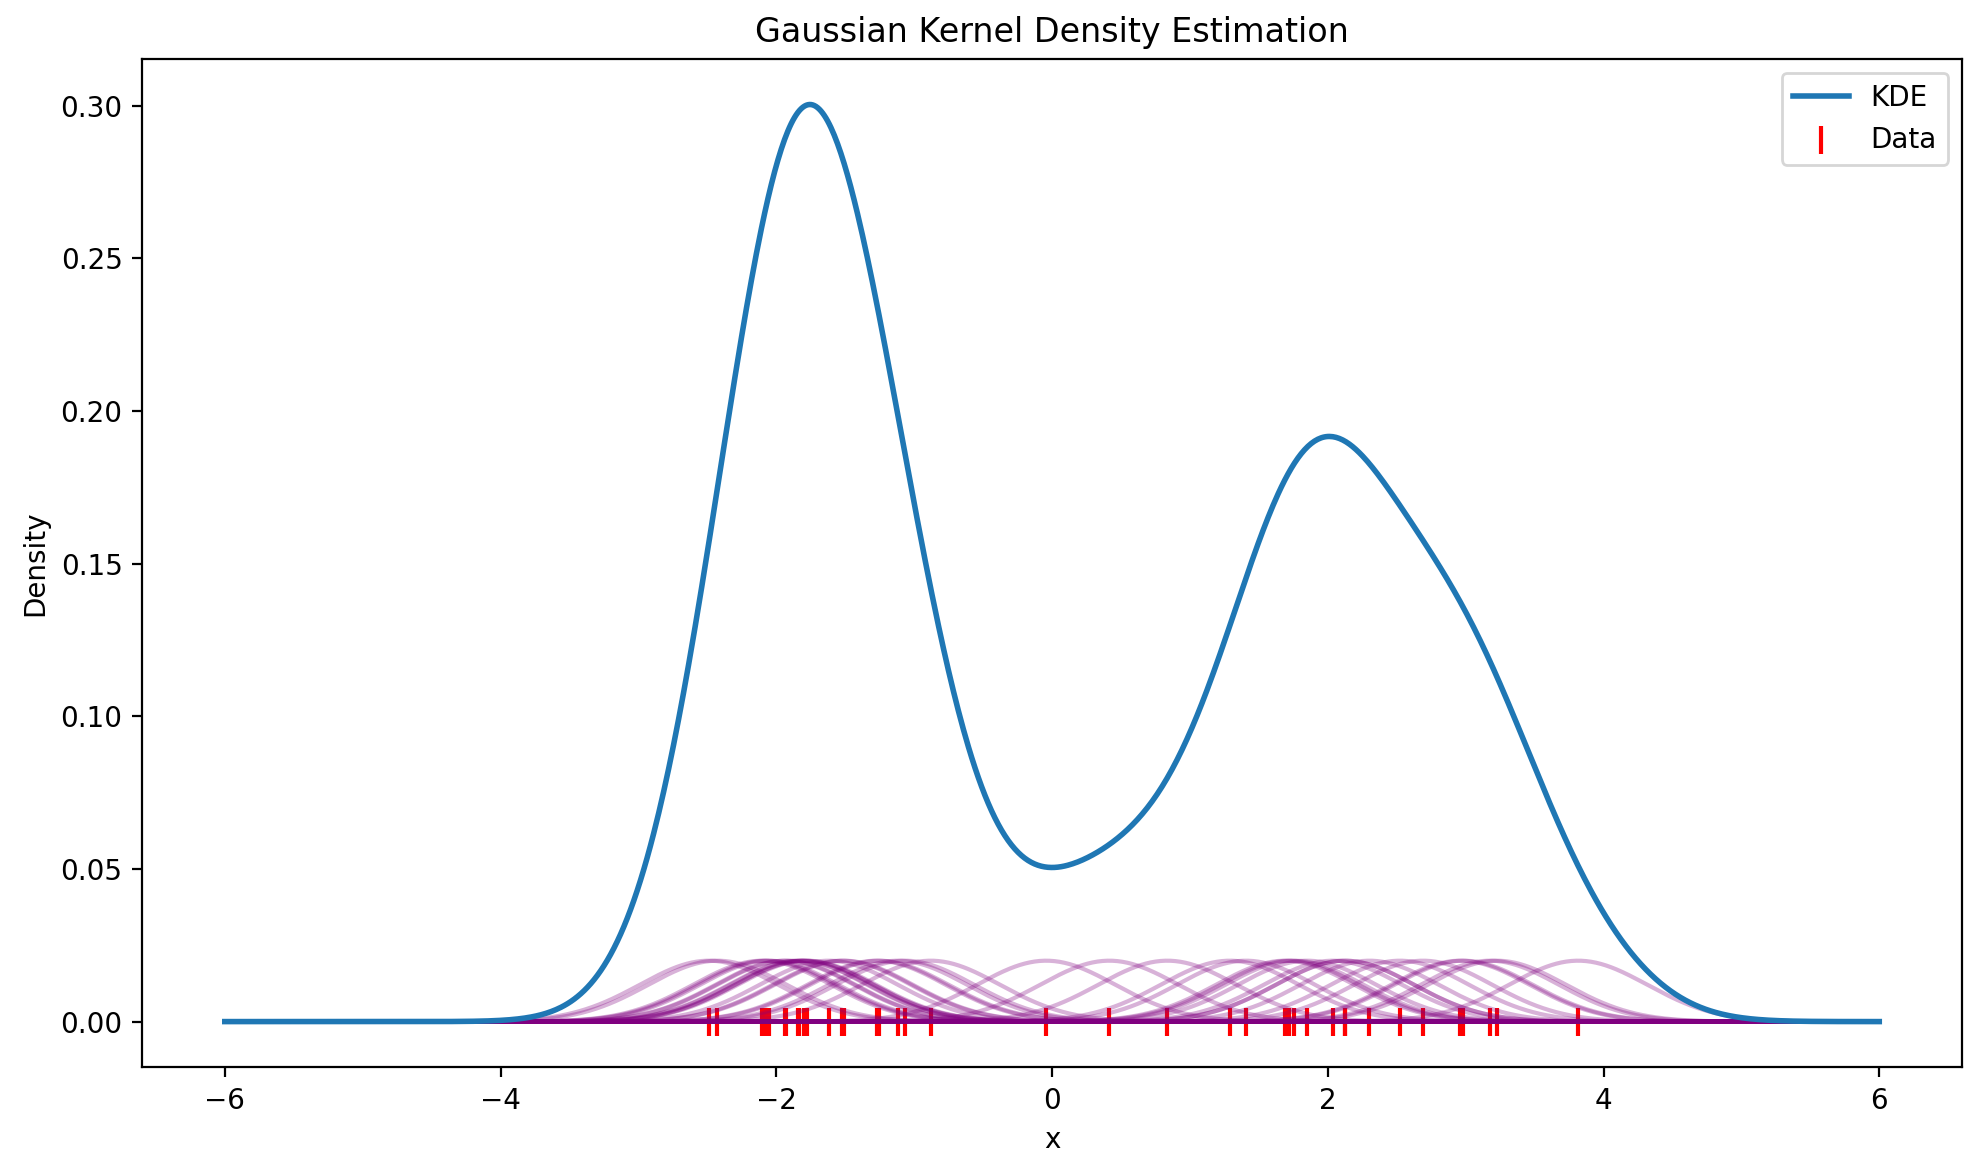
\includegraphics[width=.6\textwidth]{images/gaussian_kde} 
\end{figure}
%\bottomtext{Reference: Bishop Sec 20.3.2}
\end{frame}



\begin{frame}{From score matching to diffusion}
\small 
Using a Gaussian KDE, the score-matching loss function for a neural network with weights $\+w$ becomes:

\begin{align*}
\only<1->{J(\+w) &= \half \int \norm{ \explaintermbrace{estimated score}{\+s_\+w(\+z)} - \explaintermbrace{``true'' score}{\nabla_\+z \ln q_\sigma (\+z)}}^2 \labeledbluemathbox{KDE}{q_\sigma(\+z)} \text{d}\+z  \\} 
\only<2-4>{  &= \half \int \int \norm{\+s_\+w(\+z) - \labeledgreenmathbox{kernel score}{\nabla_\+z \ln q_\sigma (\+z \mid \+x)}}^2 \labeledpurplemathbox{kernel}{{q_\sigma(\+z \mid \+x)}} \labeledredmathbox{true density}{p(\+x)} \text{d}\+x \text{d}\+z \\} 
\only<3->{  & \approx \frac{1}{2N} \sum_{n=1}^N \int \norm{\+s_\+w(\+z) - \labeledgreenmathbox{kernel score}{\nabla_\+z \ln q_\sigma(\+z \mid \+x_n)}}^2 \labeledpurplemathbox{kernel}{q_\sigma(\+z \mid \+x_n)}   \text{d}\+z} \\
\only<3->{ & \qquad \qquad \qquad \qquad \text{ where } \+x_n \sim \labeledredmathbox{true density}{p(\+x)} }
\end{align*}
%

\only<4>{\textbf{Remarks.} All equalities are up to a constant in $\+w$. The second equality is from Vincent (2011). The third is Monte Carlo approximation. Reference: Bishop Sec 20.3.2.
}

\only<5->{Now compute $ \greenmathbox{\nabla_\+z \ln q_\sigma(\+z \mid \+x_n)}$ under a diffusion model, whose multistep kernel is $\purplemathbox{q_\sigma(\+z \mid \+x_n)} = \N\big(\sqrt{\alpha_t} \+x_n \; , \; (1-\alpha_t) \+I \big)$.
}

\only<6->{
Solution: $ \greenmathbox{\nabla_\+z \ln q_\sigma(\+z \mid \+x_n) = -\frac{1}{\sqrt{1-\alpha_t}} \+\epsilon}, \qquad \text{ where }   \+\epsilon \sim \N(\+0,\+I)$.
}

\only<7->{\colorbox{yellow!30}{\textbf{Poll.}} So what?} \only<8->{We are training the model to \textbf{\qq{predict the noise}}, just like diffusion!!!
}


\end{frame}


\begin{frame}[standout]

Big Question: \\
\vspace{1in}
What are the advantages of bringing in SDE's to generative modeling? 

\end{frame}


\section{Lightning Chat}

\begin{frame}[standout]
\href{https://docs.google.com/presentation/d/1TuzM_z8jy-vL0edholKLbP3a4b6cbZc7Y9Yq_zwJUcY/edit}{\alert{\underline{Lightning Chat}}}
\end{frame}




\section{Tempest Overview}

\begin{frame}[standout]
Tempest Overview
\end{frame}






\end{document}

